\documentclass[14pt, fleqn, xcolor={dvipsnames, table}]{beamer}
\usepackage[T2A]{fontenc}
\usepackage[utf8]{inputenc}
\usepackage[english,russian]{babel}
\usepackage{amssymb,amsfonts,amsmath,mathtext}
\usepackage{cite,enumerate,float,indentfirst}
\usepackage{cancel}
\usepackage{graphicx}
\usepackage{animate}
\usepackage{ulem}

\usepackage{tikz}
% \usepackage{enumitem}
\usetikzlibrary{shadows}

% \usepackage{enumitem}
% \setitemize{label=\usebeamerfont*{itemize item}%
%   \usebeamercolor[fg]{itemize item}
%   \usebeamertemplate{itemize item}}

\graphicspath{{images/}}

\usetheme{Madrid}
\usecolortheme{seahorse}
\renewcommand{\CancelColor}{\color{red}}

\setbeamercolor{footline}{fg=Blue!50}
\setbeamertemplate{footline}{
  \leavevmode%
  \hbox{%
  \begin{beamercolorbox}[wd=.333333\paperwidth,ht=2.25ex,dp=1ex,center]{}%
    И. Кураленок, Н. Поваров, Яндекс
  \end{beamercolorbox}%
  \begin{beamercolorbox}[wd=.333333\paperwidth,ht=2.25ex,dp=1ex,center]{}%
    Санкт-Петербург, 2014
  \end{beamercolorbox}%
  \begin{beamercolorbox}[wd=.333333\paperwidth,ht=2.25ex,dp=1ex,right]{}%
  Стр. \insertframenumber{} из \inserttotalframenumber \hspace*{2ex}
  \end{beamercolorbox}}%
  \vskip0pt%
}
\newcommand\indentdisplays[1]{%
     \everydisplay{\addtolength\displayindent{#1}%
     \addtolength\displaywidth{-#1}}}
\newcommand{\itemi}{\item[\checkmark]}

\newenvironment{mydescription}[1]
  {\begin{list}{}%  
   {\renewcommand\makelabel[1]{\color{blue}##1:\hfill}%
   \settowidth\labelwidth{\makelabel{#1}}%
   \setlength\leftmargin{\labelwidth}
   \addtolength\leftmargin{\labelsep}}}
  {\end{list}}

\title{GBDT. Смешанные модели. \\\small{Немного о работающих алгоритмах}}
\author[]{\small{%
И.~Куралёнок,
Н.~Поваров}}
\date{}
\begin{document}

\begin{frame}
\maketitle
\small
\begin{center}
\vspace{-60pt}
\normalsize {\color{red}Я}ндекс \\
\vspace{80pt}
\footnotesize СПб, 2014
\end{center}
\end{frame}

\begin{frame}{Как сделать работающие леса}{сугубо личное мнение}
\begin{itemize}
  \item Научиться работать с произвольными целевыми функциями, чтобы подбирать их под задачу
  \item Скрестить bagging и boosting
  \item Научиться строить деревья с учетом информационного prior и поправки на дисперсию
  \item Учесть особенности решающей функции в процессе обучения
  \item Сделать деревья более ``стабильными''
\end{itemize}
\end{frame}

\section{Gradient Bossted Descision Trees}
\small
\begin{frame}{Случай произвольной целевой функции}
В прошлый раз мы смотрели на AdaBoost, но он для классификации. Хотим для чего угодно. Для этого нужно научиться делать все для любого T. J.~Friedman и ко. предложили делать двухфазно:
\begin{enumerate}
  \item Берем частные производные по всем точкам лерна  $\frac{\partial T}{\partial x_i}\left(X,H_t\right)$ при текущем решени $H_t$.
  \item Построенные значения используем в качестве целевых для очередного CART:
  $$
  h_{t+1} = \arg \min_{h \in CART} \sum_i \left\|h(x_i) - {\partial T \over \partial x_i}\right\|
  $$
\end{enumerate}
После этого, очередное дерево добавляется к решению с shinkage параметром $w$: $H_{t+1}(x) = H_t(x) + w h_{t+1}(x)$
\end{frame}

\begin{frame}{Случай произвольной целевой функции}{Интерпретация}
На самом деле, мы пробуем разложить решение в функциональном пространстве деревьев таким образом:
$$
\hat{F} = \sum_{h \in CART} w_i h(x) 
$$
при этом мы жадные, и с каждым шагом стараемся быть как можно ближе к цели по всем известным точкам сразу:
$$
\arg \max_{h \in CART} \sum_i T(y_i, H_t(x_i) + w h_{t+1}(x_i))
$$
Как можно видеть, это минимизация по всем частным производным, взвешанных равновесным Евклидом\footnote{что может быть не оптимально, как мы покажем ниже}.
\end{frame}

\section{Глубина деревьев}
\begin{frame}{VC оценка для Boosting}{по Robert Schapire}
Для классификатора:
$$
P(y \ne H(x) | T) < P(y \ne H(x) | L) + O\left(\sqrt{T d \over m}\right)
$$
Для регрессии:
$$
P(\|y - H(x)\| < \theta | T) < P(\|y - H(x)\| < \theta | L) + O\left(\sqrt{d \over m \theta^2}\right)
$$
\end{frame}

\begin{frame}{Выводы о структуре обучения}
$$
P(\|y - H(x)\| < \theta | T) < P(\|y - H(x)\| < \theta | L) + O\left(\sqrt{d \over m \theta^2}\right)
$$
\begin{itemize}
  \item Размер дерева определяется минимальным необходимым уровнем взаимодействия факторов
  \item Длинные ансамбли переобучаются по корню
  \item Длинна ансамбля может быть скомпенсированна размером обучающей выборки
  \item[~]
  \item[\color{blue}$\Rightarrow$] Умеренные пеньки рулят
\end{itemize}
\end{frame}

\begin{frame}{Стабильность работы GBDT}{в зависимости от целевой функции}
\end{frame}

\begin{frame}{Стабильность работы GBDT}{выводы}

\end{frame}

\section{Смешанные модели}

\begin{frame}{Bootstrapping в процессе бустинга}
Соображения, лежащие в основе бустинга и бэггинга комплиментарны, поэтому мы можем их использовать одновременно. В частности, в оригинальном алгоритме Фридмана, на каждом шаге boosting'а, делается bootstrapping по точкам (правда там делается jackknife AFAIK).
$$
h_{t+1} = \arg \min_{h \in CART} \sum_i w_i \left\|h(x_i) - {\partial T \over \partial x_i}\right\|
$$
Такой фокус дает на наших данных ~1\% за бесплатно. Почему?
\end{frame}

\begin{frame}{BagBoo}
\begin{center}
\includegraphics[width=0.5\textwidth]{BagBoo.png}
\end{center}
\begin{itemize}
  \item Работает лучше, начиная с определенной длины ансамбля (лучше чем бустинг аналогичной длинны)
  \item Модель получается сильно больше (в 10 раз, например), поэтому годится только для соревнований
\end{itemize}
\end{frame}

\begin{frame}{Распределение трудоемкости в GBDT}
С практической точки зрения, решение задачи состоит из следующих интенсивных этапов:
\begin{itemize}
  \item Вычисление частных производных ($O(g(m))$)
  \item Подбор CART или другого дерева ($O(N m)$)
  \item Апдейт состояния для всех точек $H_{t+1}(x_i)$ (O(g(m)))
\end{itemize}
Как это не странно, но первый этап становится очень тяжелым, особенно по мере оптимизации построения дерева и усложнения $T$.
\end{frame}

\begin{frame}{BooBag}
\begin{center}
\includegraphics[width=0.5\textwidth]{BooBag.png}
\end{center}
\begin{itemize}
  \item Работает не хуже
  \item Нет ограничения с которого все работает
  \item Требует значительно меньшего количества вычислений производной
\end{itemize}
\end{frame}

\section{Деревья, которые работают}

\begin{frame}{Еще раз о информации в дереве}
Сколько всего информации в дереве:
\begin{itemize}
  \item Информация о способе разбиения в каждом ноде: $\log(n + 1) + \log(|f_l| + 1)$
  \item Информация о получившемся разбиении: $\sum_{l \in L} \frac{|l|}{|X|} \log (|l| + 1)$
  \item Значения в листьях: $|L|\times32bit$
\end{itemize}
$\Rightarrow$ Круто оптимизировать разбиения фичи (не знаем как делать) \\
$\Rightarrow$ Мы можем построить prior по тому, сколько в дереве информации (сага о $\log$)
\end{frame}

\begin{frame}{Деревянная регуляризация}{Сага о $log(n)$}
$$\begin{array}{rl}
L =& \arg \min_L \sum_{l \in L} \left(\sum_{x \in l}(x - \bar{x}_l)^2 + \lambda \frac{|l|}{|X|} \log(|l| + 1)\right) \\
= & \arg \min_L \sum_{l \in L} \left(\sum_{x \in l}(x - \bar{x}_l)^2 - x^2+ \lambda \frac{|l|}{|X|} \log(|l| + 1)\right) \\
= & \arg \min_L \sum_{l \in L} \left(- \frac{\left(\sum_{x \in l}x\right)^2}{|l|} + \lambda \frac{|l|}{|X|} \log(|l| + 1)\right) \\
\simeq & \arg \min_L \sum_{l \in L} \left(- \frac{\left(\sum_{x \in l}x\right)^2}{|l|}\right)\left(1 + \lambda \log(|l| + 1)\right) \\
\end{array}$$
У меня $\lambda = 2$
\end{frame}

\begin{frame}{Диалоги о дисперсии}
\small
В случае MSE минимизируем суммарную дисперсию на каждом сплите. Дисперсия растет с числом точек, нам интересно, что будет на бесконечности.
\begin{center}
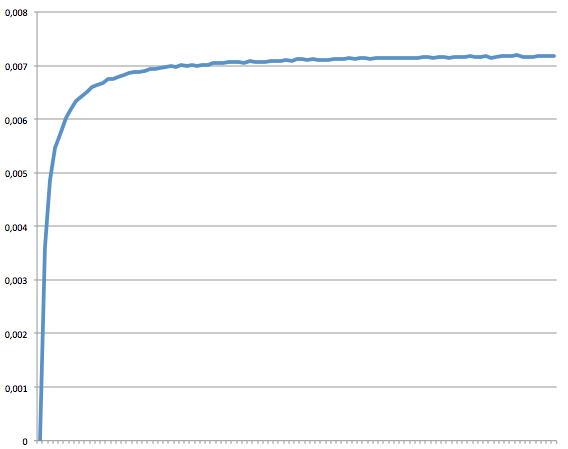
\includegraphics[height=0.5\textheight]{D.png} 
\end{center}
Можно использовать исправленную дисперсию, но помогает не всегда и есть варианты.
\end{frame}

\begin{frame}{Исправление дисперсии}
Собственно варианты. Исправленную дисперсию колбасит, а мы хотим почти всегда снизу. Можно взять 2 соседние точки на предыдущем графике и найти форму в виде
$$
a\left(n \over n + b\right)
$$
И посмотрим куда оно сойдется. Использованное значение брать в качестве дисперсии. У меня получилось так:
$$
D_{corr} = \frac{n (n - 2)}{n^2 - 3n +1} D
$$
\end{frame}

\begin{frame}{Итого}
Для того, чтобы найти каждое биение я провожу такую оптимизацию (текущий рекорд без учета попыток TN):
$$
\arg \min_{L} \sum_{l \in L} \left(- \frac{\left(\sum_{x \in l}x\right)^2}{n}\right)\frac{n (n - 2)}{n^2 - 3n +1} \left(1 + 2 \log(n + 1)\right)
$$
где $n = |l|$.
\end{frame}

\begin{frame}{Я.ЗабывчивыеДеревья}{от Cliff Brunk \& Андрей Гулин}
\begin{center}
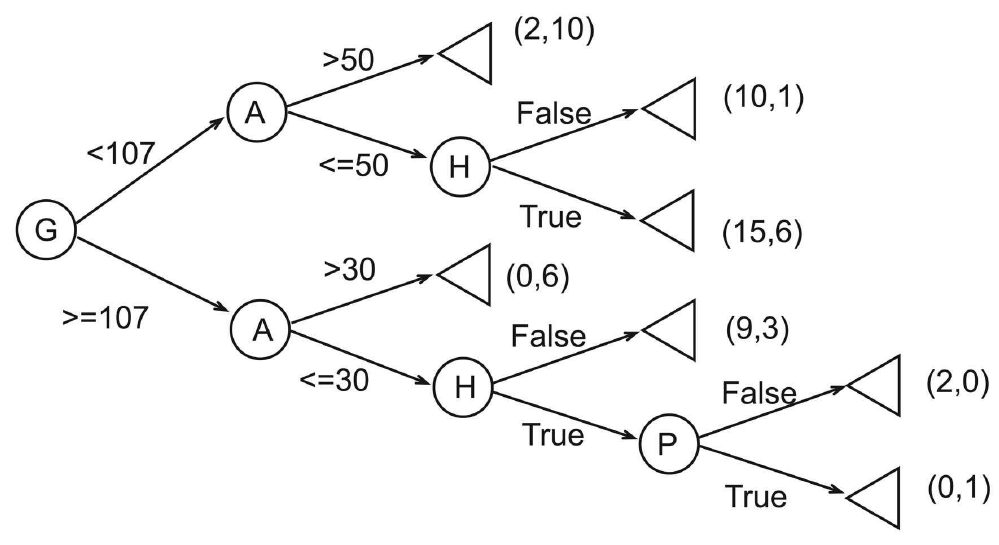
\includegraphics[height=0.3\textheight]{ObliviousTree.png} 
\end{center}
О забывчивых деревьях мы немного говорили, однако в Я, мы пошли чуть дальше:
\begin{itemize}
  \item Сделали предварительную бинаризацию: $X \to \mathbb{R}^n \to \{0, 1\}^N$
  \item На каждом уровне можно выбрать только одну \_бинарную\_ фичу.
\end{itemize} 
\end{frame}

\section{Парные производные}

\begin{frame}{Парные производные от Андрея Гулина}{или как устроен -F/-U}
$$
\arg \min_{\delta x} \sum_{(i,j)} w_{ij} \left[ \left( \delta x_i + \frac{1}{2} \frac{e^{x_j}}{e^{x_i} + e^{x_j}} \right)^2 + \left( \delta x_j - \frac{1}{2} \frac{e^{x_j}}{e^{x_i} + e^{x_j}} \right)^2 \right]
$$
$$
\mathbb{L} = \sum_{ij} w_{ij} \left(c_{leaf(d_i)} - c_{leaf(d_j)} + \frac{e^{x_j}}{e^{x_i}+e^{x_j}}\right)^2
$$

\end{frame}

\section{Заключение}

\begin{frame}{Что мы сегодня узнали}
\begin{itemize}
  \item Как раскладывать целевую функцию в ряд деревьев
  \item Какие характеристики важны в бустинге
  \item Как играть в гольф из лука
  \item Можно ли сделать еще более работающие деревья
  \item Подробности решающей функции можно использовать для еще более точного разложения
\end{itemize}
\end{frame}

\end{document}
